\documentclass[11pt, oneside]{article} 
\usepackage{geometry}
\geometry{letterpaper} 
\usepackage{graphicx}
	
\usepackage{amssymb}
\usepackage{amsmath}
\usepackage{parskip}
\usepackage{color}
\usepackage{hyperref}

\graphicspath{{/Users/telliott/Github/number_theory/png/}}
% \begin{center} \includegraphics [scale=0.4] {gauss3.png} \end{center}

\title{Primes}
\date{}

\begin{document}
\maketitle
\Large

\subsection*{prime numbers}
Positive integers larger than $1$ are of two types.  

$\circ$ \ a prime number $p$ has only two factors, $p$ and $1$

$\circ$ \ a composite number has at least one additional factor.  

Either the number is a perfect square of a prime, or it has at least two additional factors.

The first few primes are:
\begin{verbatim}
2 3 5 7 11 13 17 19 23 29 ...
\end{verbatim}

Primes are common among the small positive integers.  $A_n$ denotes the number of primes $\le n$.  $A_{10} = 4$ and $A_{100} = 24$.  The distribution is given approximately by 
\[ A_n \approx \frac{n}{\log n} \]
so $A_{1,000,000}/n \approx 0.16$.

\subsection*{The sieve of Eratosthenes}

Eratosthenes is famous in mathematics for his "sieve" which allows one to determine which numbers are prime in an economical fashion.  

We take note of him in talking about the circumference of the earth.  He was a contemporary of Archimedes and became the chief librarian at the Library of Alexandria when he was only about 35 years old.

The sieve operates by first writing down all the integers to some upper limit (here $120$).  To do things manually it is convenient to use rows with $10$ values, so there are $12$ rows in all here.  Most of the boxes have not yet been numbered (below, left).

Starting with the first prime number, $2$ (red), eliminate all the numbers divisible by $2$ (all the even numbers).  Here this has been done by coloring red all of the squares in the even numbered columns (all numbers ending in $2,4,6,8,0$).

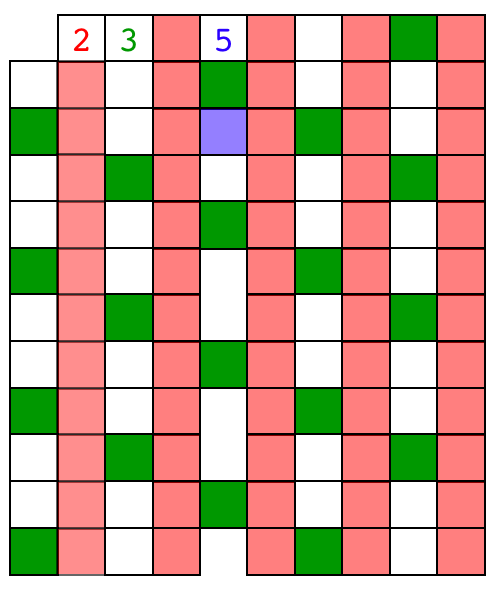
\includegraphics [scale=0.40] {sieve6.png}
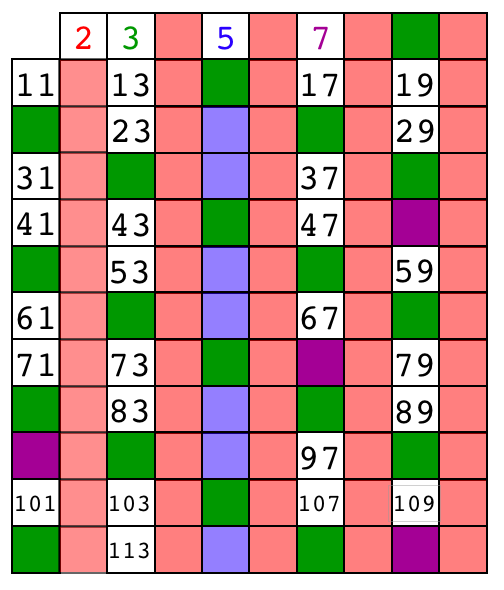
\includegraphics [scale=0.40] {sieve7.png}

Next, do the same thing with $3$ (green).  $6$ was already eliminated previously, but odd multiples of $3$ like $9$, $15$ and $21$ go away at this step.

The next larger number that still has a white square is $5$.  All the squares eliminated are white ones in the fifth row. The first value specifically eliminated at the $5$ step is $25$.  Continue with $7$, eliminating $49, 77, 91$ and $119$.

The sieve ends when the number for the beginning of the next round, the smallest number not yet eliminated, is larger than the square root of the upper limit (here $\sqrt{120}$).  So $7$ is used for the last round, because after that round the smallest remaining integer is $11$, but we terminate since $11^2 = 121 > 120$.

The graphic shows all the numbers which have yet to be eliminated after the round of $7$.   All of these numbers, $11$, $13$, $17$, and so on, as well as those used as divisors for each round of the sieve ($2, 3, 5, 7$), are prime numbers.

By testing for division by $2, 3, 5$ and $7$, we have found the first $30$ prime numbers.

From a performance standpoint, it is important that we do not need to carry out division.  All that is really needed is repeated addition.  Coding this algorithm in, say, Python is a good challenge.  A bigger challenge is to come up with a method to \emph{grow} the list of primes on demand.  This can be done by keeping track of the first value to be tested above the limit, for each prime in the current list.

\subsection*{infinite primes}

Euclid has a proof that the number of primes is infinite.

The proof is by contradiction:

Suppose the set of primes is finite, and that $p_1$, $p_2 \dots p_n$ are all of the primes.  Construct the following numbers:
\[ P = (p_1 \times p_2 \times \dots p_n)  \]
\[ Q = P + 1 \]
For a prime number $p$ to divide $Q$, it must divide the difference between $Q$ and $P$.  But that difference is $1$ and so can't be divided evenly by any prime.

Therefore, none of the known primes divides $Q$, and either

$\circ$ \  $Q$ is a prime not in the set of known primes

$\circ$ \ the set was originally incomplete.

In either case, the assumption that the set of primes is finite leads to a contradiction.

$\square$

Even for a relatively small number of primes, the second case may hold.  Start with the first prime:  $2$:
\[ 2 + 1 = 3 \]
$3$ is prime.  So then:
\[ 2 \cdot 3 + 1 = 7 \]
$7$ is prime.  So then
\[ 2 \cdot 3 \cdot 7 +1 = 43 \]
$43$ is prime.  So then
\[ 2 \cdot 3 \cdot 7 \cdot 43 + 1 =  1807 \]
$1807$ is \emph{not} prime.  ($13 \cdot 139 = 1807$).

\subsection*{testing primality}

A simple filter to apply first is to ask:  is the last digit in $\{ 0,2,4,6,8 \}$, i.e. is the number even?  Does the number end in $5$?  Or is the sum of the digits divisible by $3$ or $9$?

A more general observation is that all primes greater than $3$, are of the form $4k + 1$ or $4k + 3$, for integer $k$.  That's because $4k$ and $4k + 2$ are even, and $4k + 4 = 4(k + 1)$.

Any composite number $n$ has a unique prime factorization.  Its smallest prime factor $p$ has the property (proved above):
\[ p^2 \le n \]

Therefore, it suffices to check whether the prime numbers less than or equal to the square root of $n$ divide $n$.  If none does, then $n$ is a prime.

This can be improved still more

\url{https://en.wikipedia.org/wiki/Primality_test}

\begin{quote}by observing that all primes greater than $6$ are of the form $6k \pm 1$. This is because all integers can be expressed as ($6k \pm i$) for some integer $k$ and for $i = -1, 0, 1, 2, 3,$ or $4$; $2$ divides ($6k + 0$), ($6k + 2$), ($6k + 4$); and $3$ divides ($6k + 3$).\end{quote}

So, a more efficient method is to test if $n$ is divisible by $2$ or $3$, then to check through all the numbers of the form 
\[ 6k \pm i < \sqrt{n} \]

\end{document}